\documentclass[10pt,twocolumn]{article}

\usepackage[margin=0.72in]{geometry}
\setlength{\columnsep}{0.24in}
\usepackage{times}
\usepackage[round,authoryear]{natbib}
\usepackage{microtype}
\usepackage{graphicx}
\usepackage{booktabs}
\usepackage{tabularx}
\usepackage{multirow}
\usepackage{amsmath,amssymb,mathtools}
\usepackage{enumitem}
\usepackage{xcolor}
\usepackage{hyperref}
\usepackage[capitalize,noabbrev]{cleveref}
\usepackage{caption}
\usepackage{array}
\usepackage{xspace}
\newcolumntype{Y}{>{\raggedright\arraybackslash}X}

\hypersetup{
  colorlinks=true,
  linkcolor=blue!55!black,
  citecolor=green!35!black,
  urlcolor=blue!55!black
}
\captionsetup{font=small,labelfont=bf}
\setlength{\parindent}{1em}
\setlength{\parskip}{0pt}
\setlist{leftmargin=*,nosep}
\setlength{\textfloatsep}{8pt plus 2pt minus 2pt}
\setlength{\floatsep}{7pt plus 2pt minus 2pt}
\setlength{\intextsep}{7pt plus 2pt minus 2pt}
\emergencystretch=2em

\newcommand{\todoid}[2]{%
  \par\noindent\textcolor{red!75!black}{\textbf{TODO #1.} #2}\par}
\newcommand{\direct}{\textsc{Direct}\xspace}
\newcommand{\enumplain}{\textsc{Enum}\xspace}
\newcommand{\enumindex}{\textsc{Index-Enum}\xspace}
\newcommand{\native}{\textsc{Native-CoT}\xspace}
\newcommand{\R}{\mathbb{R}}
\newcommand{\E}{\mathbb{E}}
\newcommand{\eps}{\varepsilon}
\newcommand{\ind}{\mathbb{I}}
\newcommand{\logit}{\operatorname{logit}}
\newcommand{\uniq}{\operatorname{uniq}}

\title{\vspace{-1.2em}\textbf{How Does Chain-of-Thought Help Language Models Count?}\\
A Causal Test of Global Aggregation and Sequential Retrieval}
\author{Anonymous Authors}
\date{}

\begin{document}
\maketitle
\vspace{-1.2em}

\begin{abstract}
Counting sparse, semantically defined records in a long context requires a model to identify
the relevant sources, avoid duplicates, aggregate their number, and express the result.
We ask how explicit chain-of-thought (CoT) changes this computation relative to direct,
non-thinking generation. Preliminary realistic needle-in-a-haystack experiments show that
native CoT and controlled enumeration are substantially more accurate than direct answering in
the moderate-count regime, while all modes degrade with count and context length. We formulate
two competing accounts of direct counting---a record-by-record running update and a total formed
near the final query---and contrast both with a sequential CoT computation consisting of
matched-source retrieval, trace writing, progress update, and next-source or stop control.
Our evidence standard separates count decodability, update consistency, and causal use.
We then define functional scores for broad aggregation, targeted retrieval, and
progress-transition components, and specify interventions that must propagate through source
identity, unique coverage, progress-state quality, and the complete parsed answer.
The mechanism study centers on Qwen3-8B and Gemma4-E4B, with a broader behavioral panel and
controlled synthetic training dynamics.
\todoid{A0}{Replace preliminary language with measured effect sizes and the strongest claim
supported by the completed causal chain.}
\end{abstract}

\section{Introduction}
Language models can retrieve individual facts from long contexts yet fail to report how many
facts satisfy a semantic predicate. This sparse-record counting task is useful because an exact
answer depends on several separable operations: semantic matching, coverage of all valid
records, duplicate avoidance, accumulation, stopping, and numerical readout. A final error alone
does not identify which operation failed.

Explicit reasoning often improves the answer, but the explanation is underspecified.
CoT could improve source selection, externalize an otherwise internal state, supply convenient
number tokens, alter the stopping policy, or simply add computation. The mechanistic question is
therefore not whether ``thinking helps,'' but:
\begin{quote}
\emph{Does CoT change the retrieval-and-aggregation computation used for counting, and which
causal step accounts for the accuracy gain?}
\end{quote}

Our working hypothesis is an \emph{algorithmic path change}. Direct answering may combine many
record contributions at the final query and read out a total from a terminal state. CoT may
instead sequentialize the task into targeted retrieval, trace writing, progress update, and
continue/stop decisions. Crucially, neither path is assumed in advance. In particular, we test
whether direct answering actually maintains a causally used running counter, and whether a
CoT progress state survives controls for visible index tokens.

This framing differs from homogeneous repeated-item counting and from systems that externally
partition the input before aggregation. Here, the same unstructured context is reused across
reasoning modes, and the relevant records are sparse semantic objects. The planned contributions
are:
\begin{enumerate}
  \item a frozen, request-level behavioral map over count, length, mode, model, and failure type;
  \item a controlled sibling-stimulus design that separates record-wise running updates from
  terminal aggregation and removes visible-index leakage from CoT progress;
  \item registered hidden-state landmarks and functional routing scores whose discovery and
  causal evaluation use disjoint prompt families; and
  \item a time-indexed intervention chain linking source identity, unique coverage, progress and
  stopping, terminal readout, and the complete parsed answer.
\end{enumerate}

\begin{figure*}[t]
  \centering
  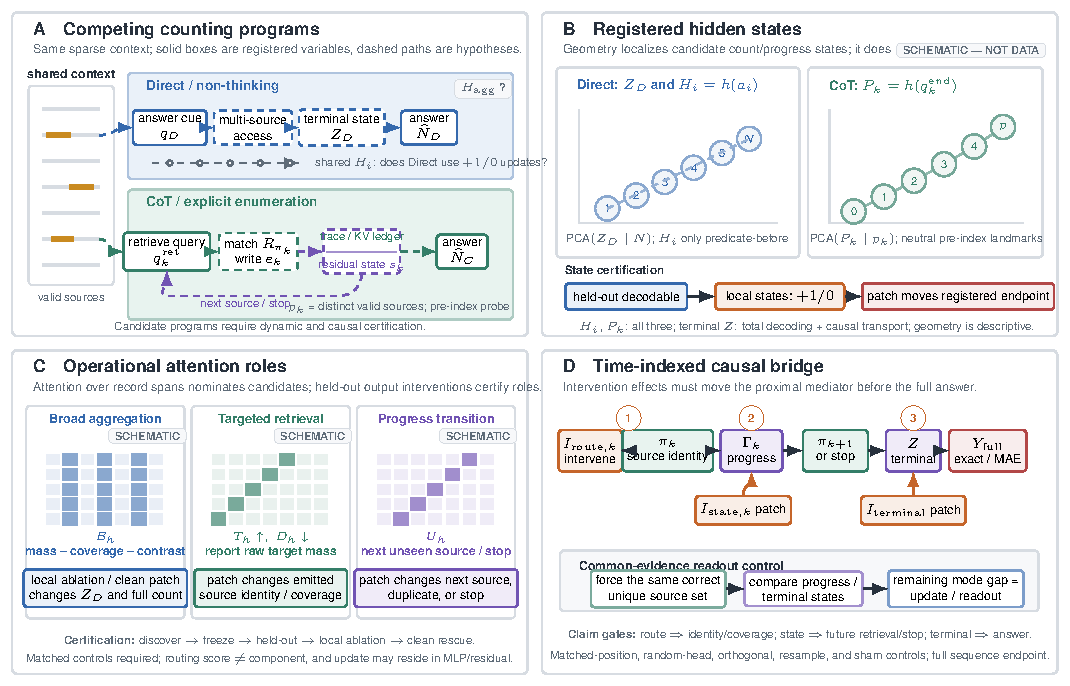
\includegraphics[width=\textwidth]{figures/mechanism_overview.pdf}
  \caption{\textbf{Mechanism map and causal test plan for Direct and CoT counting.}
  \textbf{A:} Direct answering is tested for terminal multi-source aggregation and, only in
  prompts where the counting predicate precedes the records, whether it causally uses the shared
  record-end states $H_i$. CoT is tested for a recurrent program that retrieves one matched
  record, writes evidence, updates a progress carrier, and selects the next record or stops.
  \textbf{B:} Registered hidden-state landmarks separate the Direct terminal state $Z_D$,
  predicate-conditioned record-end states $H_i$, and CoT pre-index states $P_k$. Local
  counter/progress claims require held-out decoding, the correct $+1/0$ dynamics, and a
  downstream patching effect; terminal states require total decoding and causal transport.
  \textbf{C:} Broad-aggregation, targeted-retrieval, and progress-transition candidates
  are nominated by attention scores but named functionally only after local ablation and clean
  patch rescue. \textbf{D:} Time-indexed interventions must first move the corresponding
  mediator---source identity/coverage, future retrieval or stopping, or terminal readout---and
  then the complete parsed answer. Common-evidence controls isolate update/readout from
  retrieval. All miniature trajectories and heat maps are schematic analysis templates, not
  empirical results; dashed paths are hypotheses.}
  \label{fig:overview}
\end{figure*}

\section{Experimental Design}
\subsection{Task and frozen naturalistic stimuli}
A passage contains source occurrences $R_1,\ldots,R_M$. Under a model tokenizer, occurrence
$i$ occupies the half-open token span $I_i=[s_i,e_i)$. A semantic predicate $q$ gives
\[
\begin{aligned}
  y_i&=\psi_q(R_i)\in\{0,1\},\\
  G_q&=\{i:y_i=1\},\qquad N=|G_q|.
\end{aligned}
\]
The source identity is the \emph{occurrence index} $i$, not merely the city or score string:
retrieving the same occurrence twice is a trace duplicate, whereas two distinct valid
occurrences both contribute to the count.

The behavioral suite is the frozen Realistic NIAH V2 grid. Filler text is built from a
content-deduplicated 218-source Paul Graham corpus. For each seed, essays are shuffled once and
the five length conditions use nested prefixes; an essay is never repeated to fill a context.
We cross post-insertion canonical lengths
$L\in\{2000,3000,5000,10000,20000\}$, counts
$N\in\{1,2,3,4,5,6,8,10,20,30\}$, and seeds $1234,\ldots,1243$, yielding 500 base passages.
Length is exact under the frozen Qwen3-8B tokenizer; realized length under every evaluated
tokenizer is also recorded.

Each target is a sentence of the form
\begin{quote}\small
\texttt{In the 2024 city score audit, <city> received a score of <score>.}
\end{quote}
Cities and scores are unique within a passage. Candidate insertion points are conservative
sentence endings that exclude numeric strings, URLs, paths, and common abbreviation periods.
They are sampled without replacement when enough sites exist; any replacement or word-boundary
fallback is logged rather than silently treated as an ordinary sentence insertion. The
generator then adjusts only neutral filler and regenerates until the \emph{post-insertion}
canonical length is exact. Freezing fails unless every target appears exactly once, no
target-like sentence occurs in the filler, every character span maps to a verified tokenizer
span, and no insertion is truncated. The base passage, target identities, insertion depths, and
SHA256 are frozen before mode or model expansion. Consequently, all modes and models for one
stimulus see the identical passage text.

\subsection{Controlled sibling stimuli for mechanism identification}
The naturalistic grid measures behavior but is not by itself sufficient to distinguish a local
counter from late aggregation: changing $N$ also changes how many record-like sentences are
inserted. We therefore construct a disjoint, model-audited mechanism suite. A stimulus family
\[
 \omega=(H,q,\{u_j,I_j,y_j\}_{j=1}^{K})
\]
contains the same filler $H$, $K=10$ fixed record-like slots, opaque occurrence IDs $u_j$, and
positive/negative variants that differ only in one predicate-critical attribute (balanced
across wrong-audit-type, e.g.\ \texttt{city safety audit}, and wrong-document-type, e.g.\
\texttt{city score report}, hard negatives; year alone is never treated as negative because the
frozen predicate does not restrict year). Within each mechanism model, rejection
sampling makes every positive/negative pair equal in token length. Slots are sampled once from
ten normalized-depth strata at legal sentence boundaries, with a target minimum separation of
128 model tokens; their text, order, and positions remain fixed across all siblings at one
length. A balanced permutation assigns which $N$ slots are positive, so neither depth, hard-
negative type, nor a particular city predicts validity. Longer siblings change only neutral
filler and preserve slot order and depth strata.

Mechanism corpora are rendered separately for the Qwen and Gemma tokenizers so the
post-insertion passage length is exact and every within-model sibling retains identical
downstream token positions. Cross-model corpora share the semantic family manifest, slot
ordering, labels, and normalized depths, but are not claimed to have identical token IDs or
absolute token indices.

Two paired manipulations identify different computations. A \emph{prefix-shift} sibling swaps
an early positive and a late matched negative, preserving final $N$, $L$, and all slot
identities while changing the cumulative count between those slots. A \emph{total-shift}
sibling flips one fixed slot from negative to positive, producing $N\leftrightarrow N+1$
without changing sequence length or location. Clean/corrupt activation-patching pairs are
instances of these siblings; the complete rendered token sequence is equal length within a
model, and every modified span is stored in the manifest.

\todoid{D1}{Freeze the controlled mechanism suite at
  $N\in\{0,\ldots,6,8,10\}$. At the primary length $L=5$k, target at least 120 independent
  families assigned before capture to 60 discovery, 20 validation, and 40 locked test families;
  use a family-cluster pilot power analysis to increase, not silently shrink, the locked set.
  After all layers, heads, and thresholds are frozen, test length transfer on at least 40 new
  locked families at each of $L=2$k and $10$k. Store positive/negative siblings, prefix-shift and
  total-shift pairs, prompt and continuation token IDs, every model-specific character/token
  span, and contamination and length-alignment audits. Prefix-shift is eligible only for
  $1\leq N\leq K-1$; at $N=0$ or $N=K$, use the available one-direction total shift rather than
  inventing a swap. Use seeds disjoint from the behavioral grid.}

\subsection{Paired prompts, reasoning policy, and decoding}
The registered behavioral layout is \emph{predicate-before}: the exact common cue
``You will need to count all city-score audit records \ldots'' and its definition precede the
passage, while the response request follows it. Thus
record-end states in the existing V2 data have already seen the predicate even though the final
question is after the passage. The passage and question sentence are reused verbatim; the
remaining response-policy text and the model's frozen reasoning switch define the mode.

\begin{table*}[t]
\centering
\small
\begin{tabularx}{\textwidth}{p{0.13\textwidth}p{0.34\textwidth}p{0.17\textwidth}Y}
\toprule
Mode & Response-policy suffix & Switchable-model policy & Primary role \\
\midrule
\direct & One line, \texttt{Total: <integer>}; explicitly forbids explanation or listing &
thinking off; greedy; 64 tokens & non-thinking endpoint \\
\enumplain & Passage-order bullet list of actual \texttt{city: score} pairs, then total &
thinking off; greedy; 1536 tokens & aligned, index-free process control \\
\enumindex & Same list with ordinary numeric indices, then total &
thinking off; greedy; 1536 tokens & visible-index control \\
\native & Concise native reasoning, stop once the count is known, then the same total line &
thinking on; frozen model-specific sampling; 4096 tokens & ecological CoT condition \\
\bottomrule
\end{tabularx}
\caption{Prompt control. The common cue, passage, question, chat-template revision, and parser
are frozen within a checkpoint. Always-on reasoning checkpoints are not interpreted as
non-thinking in their nominal Direct cell.}
\label{tab:prompt-modes}
\end{table*}

In the frozen V2 layout, the mode-specific response suffix occurs \emph{after} the passage.
Under a causal mask, passage-token states therefore cannot differ across modes for the same
checkpoint and stimulus if their rendered prefixes through the passage are identical. We audit
this prefix identity after applying each model's chat template. Such states are treated as a
shared scanning substrate, not as evidence that CoT encoded a cleaner counter while reading.
The mode comparison instead registers the Direct terminal state after its suffix and the CoT
states created during trace generation. A separate \emph{policy-before} control moves the
Direct/enumeration instruction before the passage to test whether an anticipated trace can
change prompt encoding; it is never pooled with the original behavioral grid.

The mechanism study adds two controls. First, a $2\times2$ prompt-policy factorial crosses
visible instruction (Direct versus unindexed enumeration) with the Qwen/Gemma reasoning switch
(off versus on), separating trace format from the native thinking policy. Second, predicate
placement has three levels: the registered predicate-before layout, a \emph{predicate-after}
layout that moves the entire task definition after the passage, and a
\emph{predicate-repeat} layout that repeats it near generation. Predicate-after record states
cannot encode the task-specific cumulative count and form a causal-mask negative control;
predicate-repeat separates availability during encoding from instruction recency.

Activations on a fixed prefix are deterministic. For free-continuation causal endpoints, paired
clean, corrupt, and patched runs use the same generation seed (common random numbers) and retain
all parse failures and truncations. Data-generation seeds and decoding seeds are separate fields;
the ten behavioral seeds are stimulus replicates, not estimates of sampling variance. We report
both teacher-forced log likelihood of the complete registered continuation and free-generation
exactness/MAE; a first-digit logit is never the sole endpoint. Equal-length null scratchpads
control for added tokens and recurrent computation.

\todoid{D2}{Run the Qwen3-8B/Gemma4-E4B $2\times2$ instruction-by-policy control and the three
predicate-placement conditions on the locked mechanism families, plus policy-before versus
suffix-after placement. Use the same sampler, generation seed, and maximum budget within each
reasoning-toggle contrast. Freeze chat-template revisions and stop rules; hash rendered prefixes
  through the final passage token. Use at least three paired decoding seeds for stochastic
  free-continuation endpoints while retaining teacher-forced sequence likelihood as the
  variance-free endpoint. Verify that any claimed algorithmic change is not explained only by
  instruction recency, output length, or a checkpoint that reasons in every nominal mode.}

\subsection{Analysis unit, splitting, and averaging}
The atomic representation observation is
\emph{one stimulus family $\times$ one rendered prompt variant $\times$ one registered
landmark $\times$ one layer}; the independent unit for splitting and uncertainty is the
stimulus family. We do not replace these observations by cross-prompt mean states before
fitting a probe or PCA, or before a primary activation patch. All siblings---modes,
predicate placements, $N/L$ variants, and clean/corrupt
counterfactuals---are assigned to the same split by family ID. Discovery fits preprocessing and
selects layers/heads; validation freezes hyperparameters and thresholds; the test families are
opened once for the registered comparisons. Additional evaluation holds out record lexemes,
templates, and complete $(N,L)$ cells.

Let $\mathcal B$ be the stimulus families, $\mathcal V_b$ the eligible rendered prompt variants
of family $b$, and $J_{bv}$ the eligible landmarks in variant $v$. Representation losses use
\[
 \frac{1}{|\mathcal B|}\sum_{b\in\mathcal B}
 \frac{1}{|\mathcal V_b|}\sum_{v\in\mathcal V_b}
 \frac{1}{|J_{bv}|}\sum_{j\in J_{bv}}
 \mathcal L\!\left(g(h_{bvj}^\ell),y_{bvj}\right).
\]
Thus every family has unit total weight, every variant within a family has equal weight, and
multiple record or trace landmarks sum to one within a variant. PCA centering, nuisance
residualization, decoder
regularization, and count directions are fitted on discovery prompts only. Figures may show
held-out individual points and class centroids with family-cluster bootstrap intervals, but
centroids are summaries, not substituted observations. Natural-state patching uses one matched
donor prompt; a training-set mean intervention is reported only as an ablation control.
Steering is the only causal intervention whose direction is defined by a cross-prompt mean, and
that mean is estimated from paired discovery-set differences. Attention statistics are first
averaged over eligible steps within a variant, then over variants within a family, and finally
equally over families. We do not average raw hidden vectors across layers, checkpoints, token
roles, or model families.

\section{Behavioral Phenomenon}
\subsection{Outcomes and paired estimands}
Direct versus Native-CoT is the primary behavioral \emph{interface contrast}: in the frozen
suite it changes both the visible instruction and the model's reasoning policy, so it is not
interpreted as a single-variable causal effect of CoT. The two enumeration modes
separate the benefit of an explicit retrieval ledger from unrestricted native reasoning. The
  unit of pairing is the frozen 500-stimulus ID. Primary outcomes are intent-to-treat
  exact-count accuracy, signed error, absolute error, parse success, truncation, and protocol
  compliance. \emph{Exact-count accuracy} means that the last valid parsed
  \texttt{Total: <integer>} equals $N$; \emph{registered success} additionally requires the
  mode-specific output format and no length truncation. We report both and never call registered
  success ``accuracy'' without qualification.
For a trace, let $\widehat G$ be the emitted multiset of aligned source-occurrence IDs and let
$A=\widehat N-|\widehat G|$. Then
\begin{equation}
 \widehat N-N
 =\underbrace{\mathrm{FP}-\mathrm{FN}+\mathrm{Dup}}_{\text{retrieval/coverage}}
 +\underbrace{A}_{\text{aggregation/protocol}},
 \label{eq:error-budget}
\end{equation}
where $\mathrm{Dup}=|\widehat G|-|\uniq(\widehat G)|$. This identity is applied to aligned
enumerations, with
$\mathrm{FP}=|\uniq(\widehat G)\setminus G_q|$ and
$\mathrm{FN}=|G_q\setminus\uniq(\widehat G)|$. It is evaluated only when both the total and
source identities are parseable; every other trace remains an intent-to-treat parse, alignment,
or protocol failure rather than being dropped.
Mode contrasts use paired stimulus effects and stimulus-family-cluster bootstrap intervals.

\subsection{Behavior and mechanism panels}
\begin{table*}[t]
\centering
\small
\begin{tabularx}{\textwidth}{p{0.18\textwidth}X X}
\toprule
Panel & Checkpoints & Scope \\
\midrule
Behavior / optional law &
Qwen3-4B, 8B, 14B, and 32B; Gemma4-E4B; GLM-4-9B and GLM-Z1-9B;
Cogito-v1-8B; Nemotron-Nano-v2-9B; Nemotron-3-Nano-4B &
Mode effects, degradation with $N$ and $L$, family heterogeneity, and complete failure budgets.
Qwen within-family trends are primary; pooled cross-family size trends are secondary. \\
Mechanism &
Qwen3-8B and Gemma4-E4B &
Registered residual states and head outputs; steering; state, head-output, and path patching;
query-local ablation; semantic outcome analysis. \\
Synthetic dynamics &
Small causal transformers in one frozen v20-based setting with a v15-style all-sequence control &
When decodability, valid updates, causal use, and routing roles emerge during training. \\
\bottomrule
\end{tabularx}
\caption{Experimental organization. Mechanism roles are aligned by semantic function, not by
layer or head index. Models that cannot implement a registered reasoning interface remain in
the failure appendix rather than being silently removed.}
\label{tab:model-scope}
\end{table*}

In the current core slice ($N\leq10$, $L\leq10$k), the working summary reports means of
$0.580$ for \direct, $0.962$ for \enumplain, $0.971$ for \enumindex, and $0.975$ for \native
across four checkpoints. These values remain explicitly preliminary until \textsc{B0} verifies
the metric label and source version for every row. Individual checkpoints are heterogeneous:
the present evidence supports a broad advantage for trace-generating interfaces, not a claim
that Native-CoT is best for every model. Current results also suggest lower accuracy and larger
absolute error as either $N$ or $L$ grows, but the interaction and coefficient stability have
not yet been established.

\todoid{B0}{Audit every requested checkpoint against the frozen stimulus hash, tokenizer and
chat-template revision, reasoning policy, generation budget, parser version, request-level
failure flags, and exact-count versus registered-success field. Preserve the per-row
\texttt{source\_version}: the current report combines formal-v2 Direct/Native rows with v2.1
enumeration replacements. Treat GLM-4-9B and GLM-Z1-9B as distinct checkpoints rather than a
same-weight thinking toggle, and record the precise reason any model/mode is not
mechanism-eligible.}

\todoid{B1}{Complete the requested behavior model set, including the missing Qwen 14B slot,
on the same 500 frozen stimuli and four registered modes. Report paired effect sizes over the
full grid and the moderate regime; intent-to-treat exact accuracy, conditional numerical
accuracy, MAE, signed error, parse/truncation/protocol failures, and
\cref{eq:error-budget}. Use stimulus-cluster bootstrap intervals and do not add predicate- or
policy-placement variants to this already frozen behavior grid.}

\subsection{Response surfaces are secondary}
We do not force a universal scaling law across dense and mixture-of-experts models with
different tokenizers and post-training. A candidate family-specific response surface is
\[
 \logit\,\Pr(\widehat N=N)
 =\alpha_{f,m}+s_{f,m}\!\left(\log L,\log(N+1)\right),
\]
where $f$ and $m$ denote family and mode. Linear, log-linear, interaction, and
shape-constrained candidates are compared on held-out stimulus families.

\todoid{B2}{Pre-register candidate surfaces and grouped train/validation/test splits. Promote
a quantitative law only if it improves held-out log loss and Brier score over a
condition-only baseline and remains stable across seeds and templates. Otherwise report
qualitative partial trends with uncertainty and move coefficient tables to the appendix.}

\section{Competing Computations}
\subsection{Minimal computation graphs}
We use minimal equations to separate what is being tested from how a particular transformer
implements it. For direct answering,
\begin{equation}
\begin{aligned}
 w_i^D&=\mathcal R_D(q,R_i),\\
 Z_D&=\mathcal G_D\!\left(\{w_i^D V_i\}_{i=1}^{M}\right),\\
 \widehat N_D&=\mathcal Q_D(Z_D).
\end{aligned}
 \label{eq:direct}
\end{equation}
$\mathcal R_D$ scores or routes record information, $\mathcal G_D$ constructs a terminal
task state, and $\mathcal Q_D$ reads out the count. Equation~\eqref{eq:direct} does not assume
that $\mathcal G_D$ is a sum, a density code, a running counter, or a single attention head.
It supports two competing hypotheses:
\begin{description}[style=nextline]
  \item[$H_{\mathrm{run}}$:] a query-conditioned state updates by approximately $+1$ after a
  valid source occurrence and by $0$ after a matched non-target, and this state affects later
  computation;
  \item[$H_{\mathrm{agg}}$:] local states may contain content or ordinal information, but the
  task-relevant total is constructed mainly near the final query through multi-record access
  and terminal readout.
\end{description}

For CoT or explicit enumeration,
\begin{equation}
\begin{aligned}
 \pi_k&=\Pi_C(q,\Gamma_{k-1}),&
 e_k&=\mathcal W_C(R_{\pi_k}),\\
 \Gamma_k&=\mathcal F_C(\Gamma_{k-1},e_k),&
 \widehat N_C&=\mathcal Q_C(\Gamma_K).
\end{aligned}
\label{eq:cot}
\end{equation}
$\pi_k$ is the source selected at step $k$, $e_k$ is the written item, and $\Gamma_k$ is the
progress carrier used to choose another source or stop. $\Gamma_k$ may combine a residual-stream
state $s_k$ with an external ledger in the visible trace and KV cache; it is not assumed to be a
scalar neural counter.

After source alignment, let
$\pi_k\in\{1,\ldots,M\}\cup\{\bot\}$ be the source-occurrence identity at trace step $k$, with
$\bot$ denoting an unaligned item. The visited set and semantic progress label are
\begin{equation}
\mathcal V_k=\uniq\{\pi_u:1\leq u\leq k,\ \pi_u\neq\bot\},
\qquad p_k=|\mathcal V_k\cap G_q|,
\label{eq:progress}
\end{equation}
the number of distinct valid sources actually retrieved. It is deliberately different from the
visible step number $k$.

\subsection{Registered token landmarks and activation capture}
Let $h_t^\ell$ be the post-block residual stream at token $t$: the output of transformer block
$\ell$ after its residual addition and before normalization by the next block. Embeddings
($\ell=0$) are diagnostic only. Every landmark is located by character-to-token offset mapping
on the \emph{final model-specific chat-rendered sequence}; no position is inferred by adding a
standalone needle length. The mechanism generator appends the same invariant end-of-record string
$D_{\mathrm{eor}}=\texttt{[END-RECORD]}$ followed by a newline to every positive and
matched-negative block. The record-end landmark is the last token whose offset overlaps the
closing bracket, and a pair is rejected unless that landmark has the same token index in both
siblings. The naturalistic V2 sensitivity analysis instead uses the final token overlapping the
target sentence's terminal punctuation.

The chat prompt is tokenized with the exact generation-time template. A teacher-forced
continuation is tokenized with its generation-time leading whitespace and no additional special
tokens, then appended as continuation token IDs; we never re-tokenize a raw prompt--continuation
string in a way that can change the final prompt token. Continuation offsets are computed on
that token axis and shifted by the frozen prompt length. A sample is rejected if the token
overlapping the \texttt{Item:} colon also overlaps the first source character, or if the token
overlapping the \texttt{Total:} colon also contains a count character. The manifest saves the
complete prompt and continuation token IDs.

\begin{table*}[t]
\centering
\small
\begin{tabularx}{\textwidth}{p{0.17\textwidth}p{0.36\textwidth}Y}
\toprule
Registered variable & Exact primary token & Label and causal role \\
\midrule
Direct local $H_i^\ell$ &
Token overlapping the closing bracket of $D_{\mathrm{eor}}$ after slot $i$;
predicate-before and predicate-repeat only &
$c_i=\sum_{j\leq i}y_j$; test target $+1$, matched non-target $0$, and downstream propagation \\
Direct terminal $Z_D^\ell$ &
Token overlapping the colon in a teacher-forced assistant prefix \texttt{Total:}, immediately
before the first count token &
Total $N$; terminal aggregation and complete-answer readout \\
CoT retrieval $Q_k^\ell$ &
Token overlapping the colon in a fixed, unindexed \texttt{Item:} marker immediately before the
source-bearing city at step $k$ &
Gold next source identity $g_k$; targeted retrieval \\
CoT progress $P_k^\ell$ &
Token overlapping the closing bracket of $D_{\mathrm{eor}}$ after the $k$th source mention and
before any next index or label &
Semantic progress $p_k$; next-source and continue/stop control \\
Controlled CoT terminal $Z_C^{\mathrm{ctrl},\ell}$ &
Token overlapping the colon in \texttt{Total:} after the canonical teacher-forced trace &
Primary terminal readout given registered evidence \\
Native CoT terminal $Z_C^{\mathrm{nat},\ell}$ &
Parsed \texttt{Total:} colon in a free-running native trace, when uniquely aligned &
Ecological replication only; never pooled with $Z_C^{\mathrm{ctrl},\ell}$ \\
\bottomrule
\end{tabularx}
\caption{Pre-registered hidden-state landmarks. Primary analyses use one token per landmark,
not a record-span average. Record-span sums are used for attention, where the estimand is source
access rather than a local state.}
\label{tab:landmarks}
\end{table*}

Writing $a_i$ for the registered record-end token, $q_k^{\rm ret}$ for the
\texttt{Item:} colon position, and $q_k^{\rm end}$ for the corresponding
$D_{\mathrm{eor}}$ landmark, the state notation is
$H_i^\ell=h_{a_i}^\ell$, $Q_k^\ell=h_{q_k^{\rm ret}}^\ell$, and
$P_k^\ell=h_{q_k^{\rm end}}^\ell$. Likewise, $q_D$ is the colon position in the
Direct \texttt{Total:} cue and $Z_D^\ell=h_{q_D}^\ell$.

Controlled CoT prefixes use the literal grammar
\texttt{Item: <city>: <score> [END-RECORD]}. The unindexed grammar is primary; numeric, random
nonnumeric, and permuted labels are placed outside the registered \texttt{Item:} and
$D_{\mathrm{eor}}$ tokens. We teacher-force all prefixes needed to create the same $k$ with
different $p_k$, then let the model continue freely for causal endpoints. Native free-running
traces are aligned to source-occurrence spans post hoc and serve as ecological replication, not
landmark discovery; parse failures remain failures.

Predicate availability, rather than the location of the final question alone, determines the
local-counter estimand. In predicate-before and predicate-repeat prompts,
\[
 c_q(t)=\sum_{i:e_i\leq t}\psi_q(R_i)
\]
is available at record endpoints. In predicate-after prompts it is forbidden by the causal
mask, so $H_i^\ell$ is used only as a query-independent content control. Terminal $Z_D^\ell$
and final-query source access are tested in all three layouts.

\subsection{When we use the word counter}
A candidate state is called a \emph{counter} only after three nested tests:
\begin{enumerate}
  \item \textbf{Decodable:} a decoder trained on disjoint prompts predicts $c_q(t)$, $p_k$, or
  $N$ from the registered state.
  \item \textbf{Dynamically consistent:} Direct decoded state changes by $+1$ after a valid
  input occurrence and $0$ after a matched non-target; CoT progress changes by $+1$ after a
  newly retrieved valid source and $0$ after an invalid or repeated source. Both tests control
  position, length, total count, density, and identity.
  \item \textbf{Causally used:} a natural-state patch or controlled steering intervention changes
  downstream source choice, progress, stopping, or the complete final answer in the predicted
  direction.
\end{enumerate}
PCA is a visualization of candidate geometry; it does not satisfy any of these tests by itself.

\section{Registered Count States and Causal Control}
\subsection{Decoding and geometry protocol}
For each layer and registered role, we fit a ridge decoder on individual discovery
prompt-landmark states with the family-equal weights defined above. Regularization is selected
on validation families. A nuisance-only model $g_0(u)$ is compared with a state-augmented model
$g_1(h^\ell,u)$; the evidence attributed to the representation is held-out improvement in MAE
and $R^2$, not raw predictability of a count that is already correlated with position.
For Direct local states,
\[
 u_D=(i,K,N,L,a_i/L,N/L,\text{depth bin},\text{template ID}),
\]
while for CoT progress,
\[
 u_C=(k,N,L,\text{trace-token length},\text{visible-label identity}).
\]
Remaining count $N-c_i$ is reported as a separate outcome rather than placed in the same
nuisance vector as $N$ and $c_i$.

For visualization, one shared PCA basis per model/layer is fitted after balancing the discovery
sample over registered role, mode, semantic label, and $(N,L)$ cell and recording the
downsampling seed. The frozen basis projects
individual locked-test states; mode-specific PCA is a sensitivity analysis. Correct and
incorrect outputs are both included in the primary fit and are separated only for a
pre-registered diagnostic. Thus a clean-looking trajectory cannot be created by averaging
states within a prompt or by selecting successful traces.

\todoid{R1}{At every landmark in \cref{tab:landmarks}, fit family-weighted nuisance-only and
state-augmented decoders for Qwen3-8B and Gemma4-E4B. Freeze preprocessing, ridge penalties,
PCA bases, and layer selection before the locked test. Report held-out incremental $R^2$/MAE,
unseen identity/template and $(N,L)$ transfer, state dispersion, and correct/error strata.
Plot individual test points plus family-cluster centroids; do not fit a projection to the
presentation prompts.}

\subsection{Direct: running update or terminal aggregation?}
For predicate-before and predicate-repeat prompts, we extract $H_i^\ell$ at all $K$ controlled
slots, not only the positive records. The primary dynamic test is a same-position
prefix-shift contrast, not the difference between two positions inside one prompt. Let siblings
$A$ and $B$ exchange a positive slot at $r$ with a matched negative at $s>r$, and let
$g_h^\ell$ be a hidden-only decoder applied after discovery-set nuisance residualization. At the
same landmark $j$,
\[
 \delta_j^\ell=
 g_h^\ell(\widetilde H_{j}^{A,\ell})
 -g_h^\ell(\widetilde H_{j}^{B,\ell})
 \stackrel{H_{\rm run}}{\simeq}
 \begin{cases}
  0,&j<r,\\
  1,&r\leq j<s,\\
  0,&j\geq s.
 \end{cases}
\]
The confirmatory region uses unchanged record blocks strictly between $r$ and $s$, so the local
token and record identity are identical while the correct prefix count differs by one. The
endpoints at $r$ and $s$ and adjacent-position increments within one prompt are secondary
content/update diagnostics. This contrast fixes final $N$, record-like block count, length, and
position and is therefore the decisive guard against total-count, density, and nuisance-only
leakage. Predicate-after states provide the causal-mask negative control.

Under the frozen suffix-after V2 layout, a successful prefix-hash audit makes each $H_i^\ell$
identical across response modes for a given checkpoint and stimulus. Hence this analysis asks
whether \direct later \emph{uses a shared scanning state}; it cannot establish that \direct
created a mode-specific state or that CoT created a cleaner one while reading. Mode-specific
passage encoding is tested only in the separate policy-before control.

For causal propagation, a total-shift clean/corrupt pair differs at one equal-length slot $r$.
The primary counter-transport patch copies a clean natural activation at the first unchanged
downstream record landmark $j>r$ into the corrupt run at the same token and continues the
forward pass. We pre-register flips with such a downstream anchor; patching the modified
record's own endpoint is retained only as an evidence-transport positive control. Endpoints are,
in order:
(i) decoded cumulative count at later slots; (ii) the terminal state $Z_D$; (iii) sequence log
likelihood after \texttt{Total:}; and (iv) the complete free-generated count. A positive-to-
positive identity patch, negative-to-negative patch, unrelated-position patch, norm-matched
random state, and clean-to-clean sham estimate nonspecific transport.

$H_{\mathrm{agg}}$ requires positive evidence and is not accepted merely because a local probe
fails. We test whether final \texttt{Total:} states and query-local multi-record routes carry
$N$, whether total-shift terminal patches move the full answer, and whether these effects remain
when local ordinal information is controlled. Evidence for $H_{\mathrm{run}}$ requires
decodability, correct $+1/0$ dynamics, and propagated local patches; evidence for
$H_{\mathrm{agg}}$ requires a selective terminal route/state intervention.

\todoid{R2}{Run the Direct prefix-shift and total-shift experiments at every frozen candidate
layer. Use same-position hidden-only contrasts at unchanged landmarks for the primary $+1/0$
test; do not treat a second valid input occurrence as a no-op. Patch single natural donors at
unchanged downstream $H_j$ and at $Z_D$ separately, with the modified-record endpoint only as an
evidence-transport control. Measure later landmarks, terminal state, complete-answer likelihood,
and free-generation exact/MAE. Include predicate-after and predicate-repeat,
identity-preserving, position, random, norm, and sham controls.}

\subsection{CoT progress without label leakage}
The CoT label is $p_k$ from \cref{eq:progress}, not the emitted step number. In passage-order
enumeration, the pre-registered next gold source is
\[
 g_k=\operatorname*{arg\,min}_{i\in G_q\setminus\mathcal V_{k-1}}s_i,
\]
where $\mathcal V_{k-1}$ is the set of source-occurrence IDs already retrieved. Gold-target
alignment is the primary estimand; attention to the source the model actually emits is reported
separately as execution alignment, so a consistently wrong retrieval does not receive a high
mechanism score. If the set is empty, the registered target is \texttt{stop} rather than a
source.

At the same visible step $k$, we teacher-force three equal-length prefixes whose newest item is:
a new gold source ($\Delta p=1$), a matched non-target ($\Delta p=0$), or a repetition of an
already visited source occurrence ($\Delta p=0$). Complementary prefixes hold $p_k$ fixed while
changing trace extent. We repeat them with no index, random nonnumeric labels, and permuted
numeric indices, always extracting at the invariant \texttt{Item:} and $D_{\mathrm{eor}}$
tokens. A state that follows $p_k$ under these transformations is evidence for semantic
progress; a state that follows $k$ or the displayed label is not.

A clean $P_k^\ell$ is patched into a matched corrupt prefix before the model chooses its next
source. The proximal endpoints are the sequence probability and free-run identity of $g_{k+1}$,
duplicate probability, and continue/stop probability; later endpoints are unique coverage,
$P_{k+1}$, and the complete count. Residual-only transport patches $P_k^\ell$ while preserving
the recipient trace/KV cache. Trace/KV-only path patching transports donor trace-token keys and
values while preserving the recipient current residual. The joint intervention tests whether
the two carriers are complementary; it is interpreted cautiously because KV transport is the
more off-manifold operation.

For geometric steering, the discovery-set direction is the normalized prompt-paired difference
\[
 v_\ell=
 \frac{\E_{\omega,k}[P_k^\ell(\Delta p=1)-P_k^\ell(\Delta p=0)]}
 {\left\|\E_{\omega,k}[P_k^\ell(\Delta p=1)-P_k^\ell(\Delta p=0)]\right\|_2}.
\]
We add $\alpha v_\ell$ only at the registered token, choose the layer and $\alpha$ range on
validation families, and compare with norm-matched random and orthogonal directions. This
cross-prompt mean defines a steering direction only; primary patching still uses a single
matched natural donor.

\todoid{R3}{Run the equal-length new-gold/non-target/repeated-source prefix experiment with
unindexed, random-label, and permuted-index interfaces. Test same-$k$/different-$p_k$ and
same-$p_k$/different-extent pairs; residual-only, trace/KV-only, and joint transport; natural
same-position patches; and a validation-selected $\alpha$ steering sweep. Report gold
next-source likelihood/identity, duplicate and stop behavior, later progress, unique coverage,
and the complete parsed count with norm-matched, random, orthogonal, position, and sham
controls.}

\subsection{State dispersion is not probe error}
Let $\widetilde h^\ell$ be the residual after a discovery-set nuisance model removes the
registered position, length, density, template, and label covariates. For semantic count or
progress $c$, define the family-equally weighted moments for each registered role separately
\[
 \mu_c^\ell=\E_{\omega}[\widetilde h^\ell\mid c],\qquad
 \Sigma_c^\ell=\operatorname{Cov}_{\omega}(\widetilde h^\ell\mid c).
\]
Let $d_c=\mu_{c+1}^\ell-\mu_c^\ell$,
$u_c=d_c/(\|d_c\|_2+\eps)$, and
$\bar\Sigma_c=(\Sigma_c^\ell+\Sigma_{c+1}^\ell)/2$. We measure conditional state dispersion
relative to adjacent separation as
\begin{equation}
 \nu_{\mathrm{state}}^\ell(c)=
 \frac{u_c^\top\bar\Sigma_c u_c}
      {\|d_c\|_2^2+\eps}.
 \label{eq:state-noise}
\end{equation}
This is a representation statistic and is reported only when adjacent separation exceeds a
validation-frozen threshold. Held-out decoder error measures accessibility to a chosen decoder
and is reported separately. We test, rather than assume, that
$\nu_{\mathrm{state}}(c)$ grows with count in Direct and is smaller at CoT progress landmarks.
Because $H_i$, $P_k$, and $Z$ inhabit different token roles, this cross-role comparison is
exploratory and cannot by itself establish an algorithmic path change.

\section{Routing and Update Components}
\subsection{Three functional scores}
Let $A_{q,t}^{\ell,h}$ be attention from query position $q$ to token $t$ for head $h$, and define
record-span mass
\[
 a_i^{\ell,h}(q)=\sum_{t\in I_i}A_{q,t}^{\ell,h}.
\]
We sum over the complete, pre-registered record span rather than selecting a favorable token
after inspecting a heatmap. Each score is computed per eligible query, averaged over queries
within a prompt variant, over variants within a family, and only then equally over families. The following scores nominate
candidates; causal criteria below determine the functional label. Because raw mass can favor a
longer city or record span, every score is accompanied by the span-density sensitivity
$a_i^{\ell,h}(q)/|I_i|$ and enrichment relative to a uniform-attention baseline.

\paragraph{Broad aggregation score.}
At the Direct answer-cue token $q_D$, let
$M_G^{\ell,h}=\sum_{i\in G_q}a_i^{\ell,h}(q_D)$ and
$r_i^{\ell,h}=a_i^{\ell,h}(q_D)/(M_G^{\ell,h}+\eps)$. For $N\geq2$, define
\[
 B_{\ell,h}=\E_\omega\!\left[
 M_G^{\ell,h}\,
 \frac{\exp\{-\sum_{i\in G_q}r_i^{\ell,h}\log(r_i^{\ell,h}+\eps)\}}{N}
 \right].
\]
The effective-coverage factor is one when gold-span mass is uniform and $1/N$ when it is
concentrated on one source. We additionally report gold-versus-matched-negative contrast; high
$B_{\ell,h}$ without contrast is nonspecific broad access. We call a high-scoring head a
\emph{broad aggregation component} only if query-local head-output ablation disrupts $Z_D$ or
the count and a clean output patch restores it.

\paragraph{Targeted retrieval score.}
At CoT retrieval step $k$, let $g_k$ be the pre-registered next gold source in passage order and
$\mathcal V_{k-1}$ the sources already present in the prefix. Define
\[
\begin{aligned}
 T_{\ell,h}&=\E_\omega\E_{k\mid\omega}\!\left[
 \frac{a_{g_k}^{\ell,h}(q_k^{\rm ret})}
      {\sum_{i=1}^K a_i^{\ell,h}(q_k^{\rm ret})+\eps}
 \right],\\
 D_{\ell,h}&=\E_\omega\E_{k\mid\omega}\!\left[
 \frac{\sum_{i\in\mathcal V_{k-1}}a_i^{\ell,h}(q_k^{\rm ret})}
      {\sum_{i=1}^K a_i^{\ell,h}(q_k^{\rm ret})+\eps}
 \right].
\end{aligned}
\]
We report raw gold-target mass alongside conditional selectivity. Attention to the source the
model actually emits is a separate execution-alignment statistic. A targeted retrieval
component must have high gold-target selectivity, low visited-source mass, and a causal effect
on the emitted source identity.

\paragraph{Progress-transition score.}
For nonterminal controlled prefixes, define
\[
 U_{\ell,h}=\E_\omega\E_{k\mid\omega}\!\left[
 \frac{a_{g_{k+1}}^{\ell,h}(q_k^{\rm end})}
      {\sum_{i=1}^K a_i^{\ell,h}(q_k^{\rm end})+\eps}
 \right].
\]
$U_{\ell,h}$ screens for a component that uses the completed step to prepare the next gold
source. Terminal prefixes are evaluated by the probability of \texttt{Total:}/stop and by
free-running stopping behavior rather than forcing a nonexistent source target. We use
\emph{progress-transition} or \emph{next-source control}, not ``successor head,'' unless
relabeling shows a token-independent $k\mapsto k+1$ OV map
\citep{gould2023successor}. The update itself may be implemented by an MLP or residual stream
even when an attention head supplies routing.

\subsection{From heatmap to functional component}
Every role follows the same validation ladder:
\[
\begin{aligned}
\text{discover} &\rightarrow \text{freeze}
                 \rightarrow \text{held-out selectivity}\\
                &\rightarrow \text{local ablation}
                 \rightarrow \text{clean patch rescue}.
\end{aligned}
\]
Attention maps are retained as interpretable summaries, but attention alone does not establish
information flow \citep{zhang2024patching}. Ablations are applied to head outputs at registered
queries---the head contribution after its value aggregation and output projection---not globally
whenever a local intervention is possible. Controls include random and same-layer heads,
attention-mass-matched heads, lexical adjacency, resample and mean ablation, an unrelated-token
local ablation, and clean-to-clean/corrupt-to-corrupt sham patches.

\todoid{H1}{On discovery families, compute $B_{\ell,h}$, $T_{\ell,h}$,
$D_{\ell,h}$, and $U_{\ell,h}$ for every layer/head in both mechanism models using the
step--variant--family aggregation above. Freeze candidates and thresholds on
validation families before the locked test; pre-register at most five candidates per role and
model and use a family-wise max-statistic permutation screen. Separate gold-target from
emitted-target alignment; plot raw span mass, contrast/selectivity, and a small number of real
test heatmaps. Apply Holm correction across the frozen causal head/endpoints, not across
post-selected heatmaps.}

\todoid{H2}{For each frozen candidate, run query-local head-output ablation, clean-to-corrupt
patching, and path patching into the registered state. Broad candidates must affect terminal
total quality; targeted candidates must first affect gold/emitted source identity; transition
candidates must first affect the next gold source, progress, or stop. Report necessity, partial
sufficiency, rescue, side effects, and every matched control on complete sequences.}

\section{Why CoT Helps: The Causal Chain}
The central result is not ``an ablation lowers accuracy.'' It is the time-indexed sequence
\begin{equation}
 I_{\mathrm{route},k}
 \longrightarrow \pi_k
 \longrightarrow \Gamma_k
 \longrightarrow (\pi_{k+1},\mathrm{stop})
 \longrightarrow Z
 \longrightarrow Y_{\mathrm{full}},
\label{eq:causal-chain}
\end{equation}
with side interventions
$I_{\mathrm{state},k}\rightarrow\Gamma_k$ and
$I_{\mathrm{terminal}}\rightarrow Z$. Here $\pi_k$ is source-occurrence identity;
coverage records misses, false positives, and repeated retrieval of the same occurrence;
$\Gamma_k$ includes the semantic progress state and any visible/KV ledger; and
$Y_{\mathrm{full}}$ is the complete registered continuation, parsed count, exactness, and
absolute error. A first-digit logit is not the primary endpoint.

Each intervention has a proximal claim gate. Corrupting a targeted-retrieval head at $Q_k$ must
first change the probability or identity of the gold next source before it is used to explain
coverage or count error. Patching $P_k$ must first change the next source, repetition, or stop
before it is used to explain the final count. Patching $Z$ may change
$Y_{\mathrm{full}}$ without changing coverage and therefore isolates terminal readout.
Clean-output rescue is evaluated beside corruption. Observational associations among coverage,
state quality, and $Y_{\mathrm{full}}$ are descriptive; causal language is reserved for these
paired activation interventions and their randomized controls.

\paragraph{Common-evidence readout control.}
Retrieval and readout must be separated without pretending that a teacher-forced list is a
natural Direct computation. We therefore give both reasoning-policy conditions the same
correct, passage-ordered evidence ledger and compare their state at the identical
\texttt{Total:} token. This common-evidence intervention holds coverage fixed and is an
auxiliary readout control:
if the mode gap disappears, the natural advantage is consistent with retrieval mediation;
if it remains, state construction or terminal readout contributes after evidence is fixed.

\paragraph{Compute and trace-content controls.}
An equal-length null scratchpad controls for extra tokens and recurrent computation.
Counterfactual traces preserve token length and grammar while inserting a matched non-target,
a repeat of an already visited source occurrence, or a false stop. A trace-length matched
correct prefix controls for merely having more KV positions. These interventions test whether
semantic trace content, rather than verbosity or index tokens, drives the benefit.

\paragraph{Noise with a measurable referent.}
In the main text, ``noise'' refers only to (i) measured retrieval/update errors in source
selection, coverage, and stopping or
(ii) conditional state dispersion in \cref{eq:state-noise}. Attention entropy is a routing
descriptor, not noise; parse, format, and truncation are behavioral failure categories.
Larger $N$ creates more opportunities for misses, duplicates, and stopping errors, but the shape
of that accumulation is estimated rather than imposed by an independent-step product model.

\todoid{M1}{On locked Qwen3-8B families, run a factorial route/state/terminal study with clean,
corrupt, rescue, and sham levels. For every intervention, report the proximal endpoint first:
gold/emitted source identity for route; next source/repeat/stop for state; complete answer for
terminal. Then report unique coverage, false positives, state quality, sequence likelihood,
exactness, and MAE with family-cluster intervals and paired randomization tests. Do not replace
this chain with a single accuracy drop or a cross-sectional mediation regression.}

\todoid{M2}{Repeat the decisive links in Gemma4-E4B and run the common-evidence readout,
equal-length null scratchpad, matched non-target, repeated-source, and false-stop controls.
Claim functional replication if the same semantic links hold even when layers and head
identities differ; otherwise state the model-specific boundary.}

\section{Cross-Model and Synthetic Tests}
\subsection{Functional replication}
Qwen3-8B and Gemma4-E4B are co-primary mechanism models because both support the required
reasoning interfaces and internal access. We do not expect identical head indices or a
one-to-one circuit map. Cross-model support means that the same registered variables and causal
links in \cref{eq:causal-chain} hold. If only Qwen supports the full chain, the main claim is
restricted accordingly and Gemma is reported as a boundary case.

\subsection{Synthetic training dynamics}
The synthetic experiments serve two roles: validating the causal analysis in a controlled model
and revealing the formation order of the same functional motifs. At dense checkpoints we track
behavior, held-out count/progress decoding, valid versus invalid update consistency, state-patch
restoration, and the $B_h$, $T_h$, and $U_h$ role scores. Decodability may emerge before causal
use; a routing motif may emerge before a stable progress state. Those temporal separations are
more informative than another final-checkpoint heatmap.

The v10 report supplies the clearest intervention vocabulary. Of the candidate final settings,
v20 is the preferred basis because it adds query-conditioned target sets, guarded corpus regions,
and a balanced count evaluation; v15 remains the all-sequence-loss control. The existing v20 run,
however, has one training seed and switches objective after step 1500. Any change near that point
is therefore an objective intervention, not evidence of a spontaneous phase transition. We do
not splice v15 and v20 checkpoints into one trajectory.

\todoid{S1}{Freeze a single v20-based generator, architecture, tokenizer, checkpoint schedule,
and loss mask. Run at least three training seeds plus an all-sequence-throughout control matched
to v15 exposure and an explicit objective-switch control. Use $N\leq10$ for direct LLM
comparability and $N=11$--30 only as extrapolation. Save dense checkpoints before and after
behavioral onset and the registered objective switch. At each checkpoint compute the same
decodable--dynamic--causal ladder and $B_h,T_h,U_h$ scores, using disjoint role-selection and
causal-report families. Keep this section in the main paper only if emergence order and causal
effects are stable across seeds; otherwise report it as supporting appendix evidence.}

\section{Related Work}
Controlled transformer studies show that counting can be implemented by different algorithms and
is sensitive to architecture, positional encoding, and optimization
\citep{golkar2024contextual,yehudai2024count,chang2025inductive,behrens2025counting}.
Studies of pretrained models report decodable count states, explicit partition-and-aggregate
strategies, and possible geometric readout bottlenecks
\citep{hasani2026understanding,hasani2026system2,garcia2026direction}.
These results motivate our evidence hierarchy: count information can be present without being
the state the model causally uses.

CoT and scratchpads can externalize intermediate computation
\citep{nye2021scratchpad,wei2022cot}. Mechanistic studies identify reusable attention motifs such
as induction and successor heads \citep{olsson2022induction,gould2023successor}, while activation
patching is sensitive to the corruption, metric, and patch location
\citep{zhang2024patching}. Our focus is the same sparse semantic context under direct and
explicit-reasoning interfaces, with source identity and unique coverage as registered mediators.

\section{Limitations}
Native reasoning traces are policy-dependent and need not faithfully expose all internal
computation. Forced-prefix and activation interventions can be off-manifold; magnitude sweeps,
natural donors, and side-effect audits are therefore required. Predicate availability and
response-policy placement change what local states can identify and may also change the
algorithm itself. The current behavioral summary also combines formal-v2 Direct/Native rows
with v2.1 enumeration replacements and contains one sampled continuation per stimulus; source
version and decoding variance must therefore be audited rather than hidden by pooling. The
semantic roles may be shared
across Qwen and Gemma even when their implementations differ, but two checkpoints cannot
establish universality. Finally, synthetic emergence is supportive only when its task and
metrics align with the LLM study.

\section{Conclusion}
The proposed paper is a causal comparison of counting computations, not a catalog of probes and
attention maps. Direct answering is tested for a record-wise running update versus a terminal
multi-record total; CoT is tested for matched-source retrieval and a semantic progress carrier.
The strongest conclusion requires interventions to propagate through source identity, unique
coverage, state quality, and the complete count. If only part of that chain is supported, the
claim will be narrowed to that part rather than treating a decodable direction as a mechanism.

\begin{thebibliography}{99}

\bibitem[Behrens et~al.(2025)Behrens, Biggio, and Zdeborov\'a]{behrens2025counting}
Freya Behrens, Luca Biggio, and Lenka Zdeborov\'a.
\newblock Counting in small transformers: The delicate interplay between attention and
feed-forward layers.
\newblock In \emph{ICML}, 2025. arXiv:2407.11542.

\bibitem[Chang and Bisk(2025)]{chang2025inductive}
Yingshan Chang and Yonatan Bisk.
\newblock Language models need inductive biases to count inductively.
\newblock In \emph{ICLR}, 2025. arXiv:2405.20131.

\bibitem[Garcia(2026)]{garcia2026direction}
Gabriel Garcia.
\newblock The right answer, the wrong direction: Why transformers fail at counting and how to fix it.
\newblock arXiv:2605.03258, 2026.

\bibitem[Golkar et~al.(2024)Golkar et~al.]{golkar2024contextual}
Siavash Golkar et~al.
\newblock Contextual counting: A mechanistic study of transformers on a quantitative task.
\newblock arXiv:2406.02585, 2024.

\bibitem[Gould et~al.(2023)Gould, Ong, Ogden, and Conmy]{gould2023successor}
Rhys Gould, Euan Ong, George Ogden, and Arthur Conmy.
\newblock Successor heads: Recurring, interpretable attention heads in the wild.
\newblock arXiv:2312.09230, 2023.

\bibitem[Hasani et~al.(2026a)Hasani et~al.]{hasani2026understanding}
Hosein Hasani et~al.
\newblock Understanding counting mechanisms in large language and vision-language models.
\newblock In \emph{CVPR}, 2026. arXiv:2511.17699.

\bibitem[Hasani et~al.(2026b)Hasani et~al.]{hasani2026system2}
Hosein Hasani et~al.
\newblock Mechanistic interpretability of large-scale counting in LLMs through a System-2 strategy.
\newblock arXiv:2601.02989, 2026.

\bibitem[Nye et~al.(2021)Nye et~al.]{nye2021scratchpad}
Maxwell Nye et~al.
\newblock Show your work: Scratchpads for intermediate computation with language models.
\newblock arXiv:2112.00114, 2021.

\bibitem[Olsson et~al.(2022)Olsson et~al.]{olsson2022induction}
Catherine Olsson et~al.
\newblock In-context learning and induction heads.
\newblock arXiv:2209.11895, 2022.

\bibitem[Wei et~al.(2022)Wei et~al.]{wei2022cot}
Jason Wei et~al.
\newblock Chain-of-thought prompting elicits reasoning in large language models.
\newblock In \emph{NeurIPS}, 2022.

\bibitem[Yehudai et~al.(2024)Yehudai, Kaplan, Ghandeharioun, Geva, and Globerson]{yehudai2024count}
Gilad Yehudai, Haim Kaplan, Asma Ghandeharioun, Mor Geva, and Amir Globerson.
\newblock When can transformers count to $n$?
\newblock arXiv:2407.15160, 2024.

\bibitem[Zhang and Nanda(2024)]{zhang2024patching}
Fred Zhang and Neel Nanda.
\newblock Towards best practices of activation patching in language models: Metrics and methods.
\newblock In \emph{ICLR}, 2024. arXiv:2309.16042.

\end{thebibliography}

\clearpage
\appendix

\section{Claim Gates}
The manuscript follows a claim ladder:
\begin{enumerate}
  \item \textbf{Behavior:} trace-generating interfaces outperform Direct under matched stimuli.
  \item \textbf{Process:} trace generation changes distinct-source retrieval, and the Direct
  total is identified as a running or terminal computation.
  \item \textbf{Representation:} registered states satisfy decodable and dynamic tests.
  \item \textbf{Component causality:} routing/update candidates selectively affect their
  semantic endpoints.
  \item \textbf{Integrated causality:} those changes propagate through coverage and state quality
  to the complete count.
  \item \textbf{Scope:} the functional chain replicates across Qwen and Gemma and emerges under
  a comparable synthetic setting.
\end{enumerate}
Failure at a level narrows all claims above it. In particular, a decodable Direct record state
without propagated patch effects is ``available ordinal information,'' not a running counter;
a CoT state that fails label controls is numeric-token scaffolding, not semantic progress.

\section{Prompt Serialization and Activation Manifest}
The frozen V2 user message is serialized in the following order:
\begin{quote}\small\ttfamily
You will need to count all city-score audit records in the passage below.\\
A city-score audit record names one city and gives that city's numeric score.\\[2pt]
<passage>\\
\mbox{[byte-identical frozen passage]}\\
</passage>\\[2pt]
How many city-score audit records are in the passage?\\
\mbox{[mode-specific response-policy block]}
\end{quote}
The response-policy block is the registered Direct, bullet enumeration, indexed enumeration, or
Native-CoT instruction summarized in \cref{tab:prompt-modes}. Mechanism contrasts save both the
raw user content and the output of the model-specific chat template; the latter, rather than the
unrendered string, determines prefix identity.

Every activation row stores
\texttt{family\_id}, model and tokenizer revisions, mode, predicate/policy placement,
raw-message and rendered-prefix hashes, complete input token IDs, source character spans,
model-specific token spans, registered landmark indices, data seed, decoding seed, and
\texttt{source\_version}. Assertions verify byte-identical passages across modes, identical
rendered token prefixes wherever a shared-prefix claim is made, equal sequence length for each
clean/corrupt pair, and no truncation before any registered endpoint.

\section{Predicate and Policy Placement Matrix}
\begin{center}
\small
\captionsetup{hypcap=false}
\begin{tabularx}{\columnwidth}{
  >{\raggedright\arraybackslash}p{0.23\columnwidth}
  >{\raggedright\arraybackslash}p{0.22\columnwidth}
  Y}
\toprule
Condition & Passage-time information & Valid use \\
\midrule
Predicate-before, suffix-after (frozen V2) &
Predicate known; visible suffix unseen; reasoning policy also unseen only if the rendered-prefix
audit passes &
Shared $H_i$ candidate when prefix identity passes; otherwise analyze within mode; mode-specific
$Z_D,P_k$ \\
Predicate-after &
Task predicate unseen &
Content/position control at $H_i$; terminal tests remain valid \\
Predicate-repeat &
Predicate known and refreshed after passage &
Separates passage-time availability from recency \\
Policy-before (mechanism only) &
Predicate and response policy known &
Tests mode-specific passage encoding \\
\bottomrule
\end{tabularx}
\captionof{table}{The causal mask and prompt serialization determine which state comparisons
are identifiable. Conditions other than the first are mechanism controls, not extra cells in
the frozen behavioral grid.}
\end{center}

\section{Auxiliary Density-Code Hypothesis}
One falsifiable implementation of $H_{\mathrm{agg}}$ is a normalized relevance statistic
\[
 \rho(N,L)=\frac{N}{N+\alpha(L-N)}+\eta.
\]
Its inverse has sensitivity
\[
 N(\rho,L)=\frac{\alpha L\rho}{1-(1-\alpha)\rho},
 \qquad
 \frac{\partial N}{\partial\rho}
 =\frac{\alpha L}{[1-(1-\alpha)\rho]^2}.
\]
This model predicts that modest error in a density-like code can be amplified by context length.
It is an auxiliary hypothesis, not the default description of Direct.
\todoid{A1}{Compare density, unnormalized magnitude, and running-update models by held-out
likelihood and by source-add/delete interventions. Retain this model only if its predicted
changes in terminal state and absolute error are observed.}

\section{Full Behavioral and Failure Tables}
\todoid{A2}{Include every attempted checkpoint, not only successful ones. For each
checkpoint/mode report intent-to-treat exact accuracy, conditional numerical accuracy, parse
failure, truncation, protocol failure, answer leakage, and invalid reasoning-mode rates. Record
the precise reason any cell is excluded from mechanism analysis.}

\section{Planned Result Figures}
\begin{enumerate}
  \item \textbf{Figure 1:} competing mechanisms, registered hidden states, operational head
  roles, and the time-indexed causal bridge (\cref{fig:overview}).
  \item \textbf{Figure 2 (TODO B1):} exact-accuracy and MAE surfaces plus failure budgets.
  \item \textbf{Figure 3 (TODO D1--D2, R1--R3):} registered-state geometry, dynamic updates, and
  natural state-patch effects on the controlled sibling corpus.
  \item \textbf{Figure 4 (TODO H1--H2):} real attention maps beside held-out ablation and patch
  effects for the three functional roles.
  \item \textbf{Figure 5 (TODO M1--M2):} intervention-to-coverage-to-state-to-answer effects,
  including the common-evidence readout control.
  \item \textbf{Figure 6 (TODO S1):} synthetic emergence order with seed uncertainty.
\end{enumerate}

\section{Reproducibility Checklist}
The final artifact will freeze model revisions, tokenizer files, chat templates, generation
parameters, separate data and decoding seeds, stimulus and rendered-prefix hashes, parser code,
character-to-token span maps, landmark definitions, intervention hooks, checkpoint IDs,
\texttt{source\_version}, and all discovery/validation/test splits. Request-level outputs are
retained rather than only aggregates. Hardware, precision, batching, memory optimizations, and
library versions are reported. Synthetic checkpoints and the exact data generator are stored
with provenance.

\clearpage
\onecolumn
\section{Detailed TODO Ledger}
\begin{center}
\small
\captionsetup{hypcap=false}
\begin{tabularx}{\textwidth}{
  >{\raggedright\arraybackslash}p{0.06\textwidth}
  >{\raggedright\arraybackslash}p{0.23\textwidth}
  Y
  >{\raggedright\arraybackslash}p{0.21\textwidth}}
\toprule
ID & Experiment & Required output and controls & Claim enabled \\
\midrule
B0 & Configuration and failure audit &
Frozen revisions/templates/budgets/parsers; request-level parse, truncation, protocol, and leakage
flags & Comparable behavioral panel \\
B1 & Paired behavior grid &
Four modes on 500 frozen stimuli and ten stimulus seeds; full requested model panel; exact count,
registered success, full error budget, provenance, and family-clustered intervals &
Robust behavioral phenomenon \\
B2 & Held-out response surfaces &
Qwen within-family primary; grouped held-out scoring; coefficient stability &
Optional empirical law \\
D1 & Controlled mechanism corpus &
Tokenizer-specific equal-length siblings; stratified slots; family-disjoint splits; audited
character/token spans and invariant delimiters &
Identifiable representation and patching tests \\
D2 & Prompt-policy controls &
$2\times2$ visible instruction by reasoning switch; predicate/policy placement; prefix hashes;
paired decoding seeds and equal-length null scratchpad &
Controlled algorithmic contrast \\
R1 & Registered-state decoding &
Grouped held-out probes; confound controls; state dispersion; correct/error split &
Count/progress representation \\
R2 & Direct dynamics and patches &
Predicate-before $+1/0$ test; prefix/total shifts; single same-position donors; predicate-after
negative control; terminal interventions &
$H_{\mathrm{run}}$ versus $H_{\mathrm{agg}}$ \\
R3 & CoT anti-leakage and state control &
No-index/random/permuted labels; residual versus trace/KV transport; steering and natural patches &
Semantic progress carrier \\
H1 & Frozen role screen &
$B_h,T_h,D_h,U_h$ discovery/test split; raw and conditional mass &
Candidate components \\
H2 & Functional component tests &
Local ablation; clean patch; path patch; semantic endpoints; matched controls &
Necessity and partial sufficiency \\
M1 & Integrated Qwen causal chain &
Route/state factorial intervention; coverage, progress, full-count endpoints &
Mechanism-to-behavior link \\
M2 & Controls and Gemma replication &
Common evidence; null scratchpad; semantic corruptions; co-primary replication &
CoT explanation and scope \\
S1 & Synthetic emergence &
Frozen v20 basis; dense checkpoints; three seeds; all-sequence and objective-switch controls &
Developmental support \\
\bottomrule
\end{tabularx}
\captionof{table}{Unified TODO ledger. B0--B1, D1--D2, R1--R3, H1--H2, and M1 are required for
the Qwen mechanism claim; M2 is additionally required for the stated Qwen--Gemma functional
replication claim. B2 and S1 determine optional law and developmental scope.}
\label{tab:todo-ledger}
\end{center}

\end{document}
